\section{On the details of estimating the remote resource} \label{appendix:one-way-method}

\subsection{The importance of accounting for wave directionality} \label{appendix:directionality}

\hline

\note{This is from the intro. Is it useful here?}

A detail that confound unifying these two approaches is the fact that wave energy flux is a directional and spatially varying quantity. This means that - in order to avoid double counting when computing the total resource - regional totals must account for the directionality by performing a line-integral. On the other hand, for site assessments involving sparsely positioned omni-directional devices (i.e., devices that absorb energy equally in all directions), wave directionality does not have a significant impact on the project’s technical potential. With this understanding and motivated by a desire to address the needs of the industry where it is now (i.e., most projects involve 10 or less devices), the first edition of the International Electrotechnical Commission’s resource assessment technical specification does not explicitly provide guidance on regional resource estimates or explicitly account for array effects \citep[]{internationalelectrotechnicalcommissionPart101Wave2015}. In other words, an assessment following IEC will report wave energy density but not wave energy potential. The IEC site assessment methodology has been developed through a consensus process that encourages widespread adoption and consistency. The methodology for regional assessments, on the other hand, has not been developed by consensus, which has led to inconsistent approaches and confusion when comparing results.

\hline

\note{Add a short intro about the importance of wave directionality here? (OWP is valuable, but `unit circle' method is bunk.)}

As the National Academy review points out, estimates of $R_r$ must account for wave directionity in order to avoid double-counting. For example, when a wave with energy density of $1 \unit{kW/m}$ crosses a $1 \unit{km}$ integration contour segment with its wave crests parallel to the segment, the total power is 1MW (upper row of Figure \ref{fig:directionality}). Likewise, when that same 1-km wide wave crosses a contour-segment with its wave crests at an angle to the integration contour, the total energy contained in the wave is still only 1 MW. The directionality coefficient corrects for fact that the length of the contour segment is longer to capture the whole 1-km wave at an angle (3 km in lower row of Figure \ref{fig:directionality}, where $\theta = 70.5 \unit{degrees}$). In the `unit circle' method described in the 2011 resource assessment $\delta$ is taken to be $1$ in all cases (directionality is neglected), which for the wave depicted in the lower row of Figure \ref{fig:directionality} gives an estimate of 3 MW crossing the contour. This is clearly incorrect since the 1-km wide wave only contains 1 MW of power, and demonstrates the importance of accounting for directionality.

\begin{figure}[ht]
    \centering
    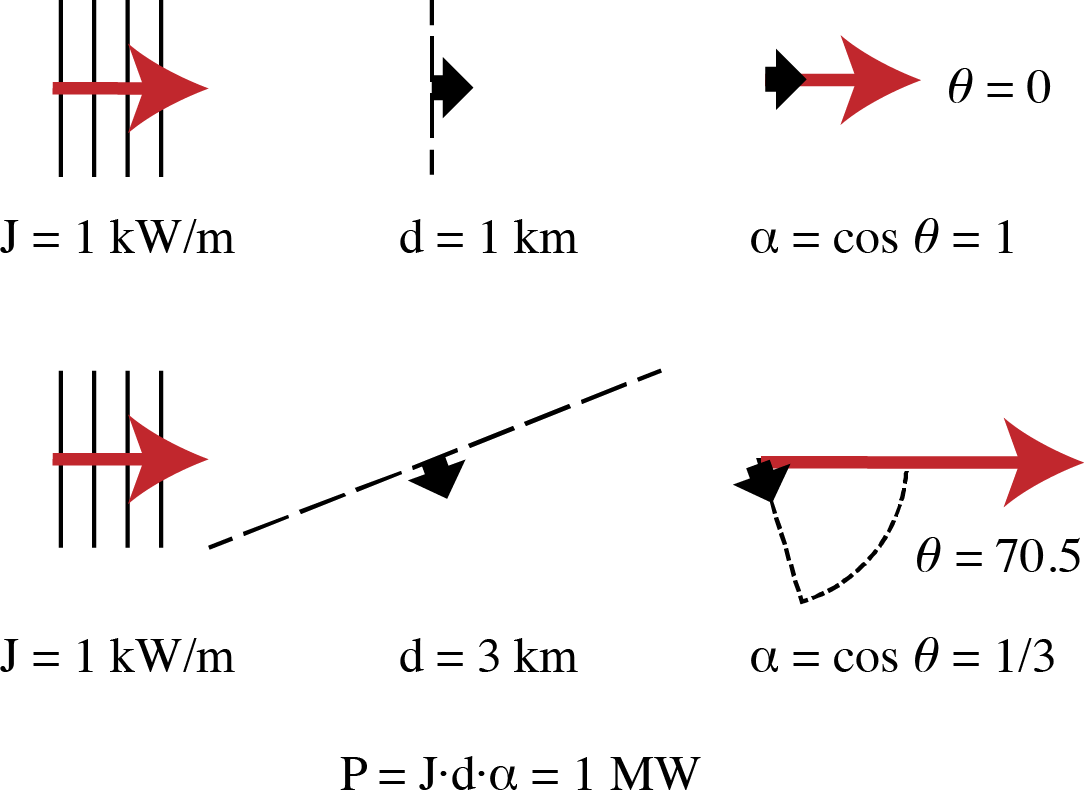
\includegraphics[width=0.6 \linewidth]{../diagram/Dot-Product_Schematic01.png}
    \caption{A diagram depicting the importance of accounting for wave directionality. The upper sequence depcits a scenario where wave crests are parallel to the integration contour ($\delta = 1$), and the lower row is a scenario where wave crests are oblique to the contour ($\delta = 1/3$). \note{I need to change the $\alpha$'s in this figure to $\delta$'s.}}
    \label{fig:directionality}
\end{figure}

One of the main reasons there has been confusion about this topic is due to the fact that many types of WECs are agnostic to the direction that wave energy arrives from (Figure \ref{fig:omni-dir}A, and \cite{EPRIwaveresource2011} ). That is, all other things being equal (wave height, period, etc.), these `omnidirectional WECs' generate the same amount of power regardless of the direction that wave energy arrives from. For a single WEC of this type, it is possible to obtain an estimate of power output by simply multiplying the device's capture-width by the omnidirectional wave power. However, when you start arranging many of these WECs together in an array where their spacing is close enough to capture all of the incident energy, then they begin to shadow one-another in a way that depends on wave direction and array-layout (i.e., in a similar manner to how wind turbine wakes reduce the performance of down-wind turbines). Accurately modeling arrays of devices is technically challenging, but the point here is that directionality matters for WEC arrays and obviously you can't get more energy out of the waves than exists in them \note{add some WEC-sim array citations here?}. For the purposes of theoretical wave resource assessment then — instead of attempting to model arrays of devices that extract all of the energy in the wave-field — we simply draw an integration contour and assume that we can extract all of the energy that crosses it (i.e., by properly accounting for directionality). 

\begin{figure}[ht]
    \centering
    \fbox{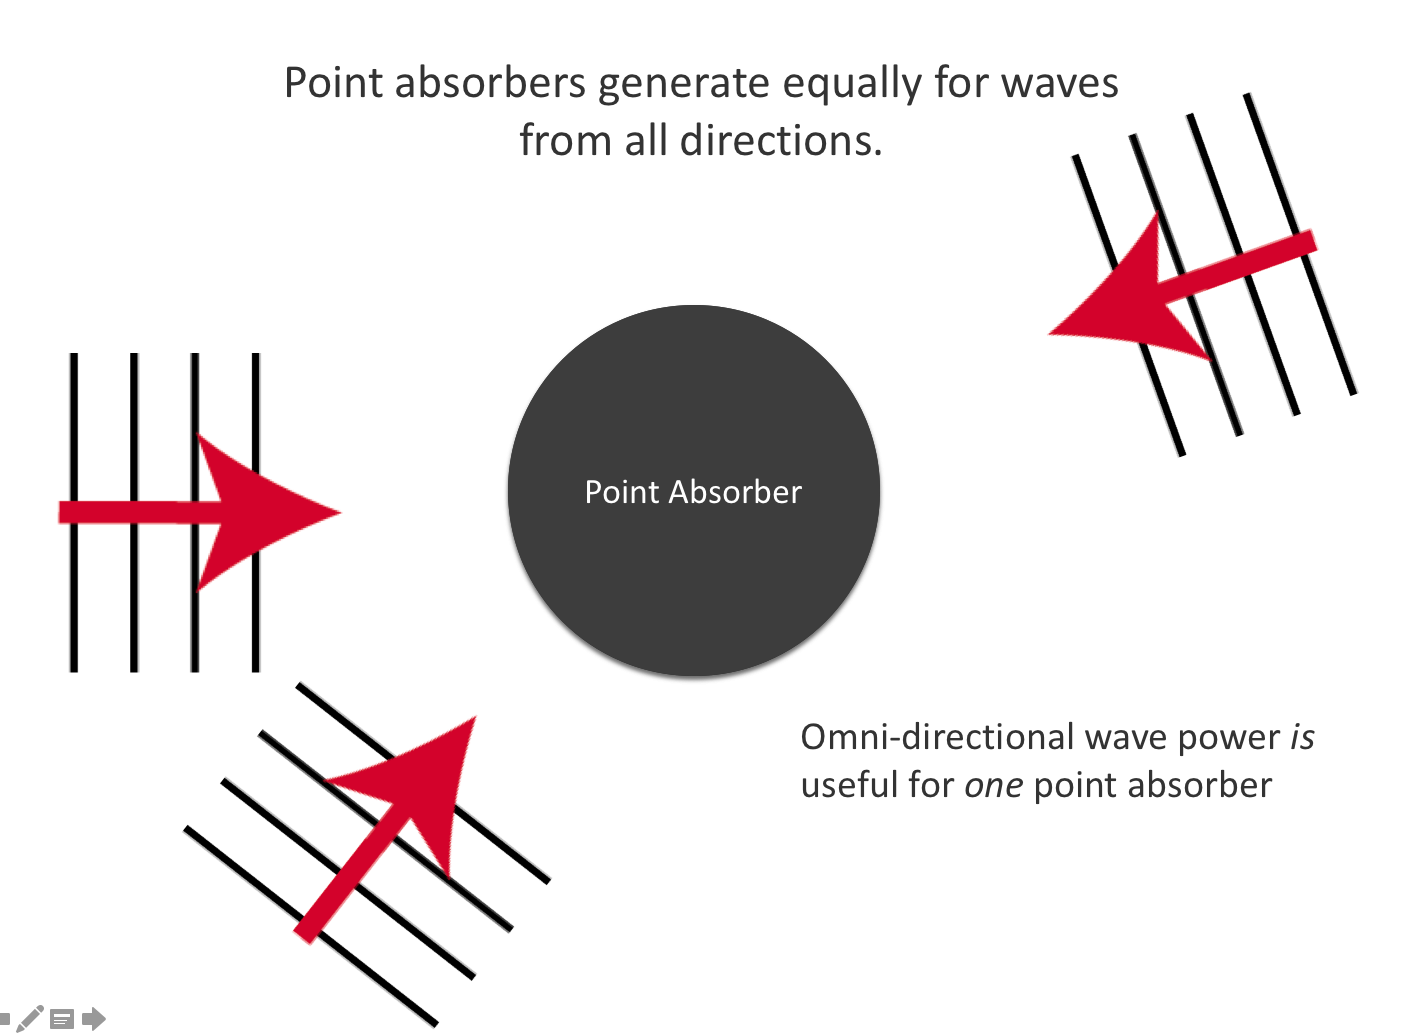
\includegraphics[width=0.3\linewidth]{../diagram/omni-dir01}}
    \fbox{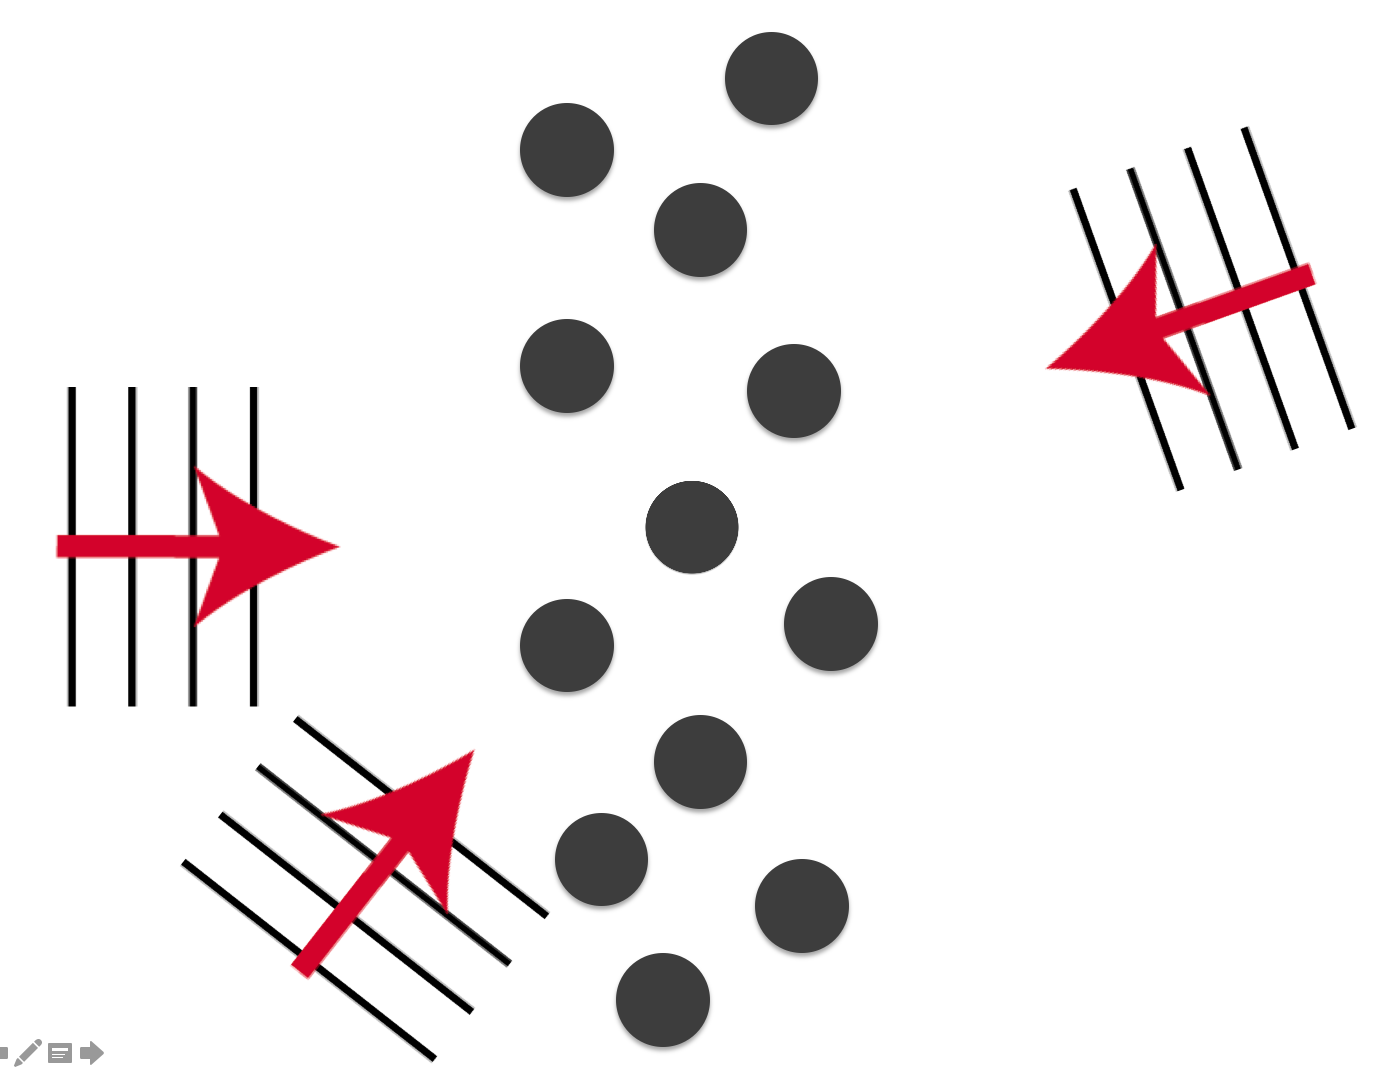
\includegraphics[width=0.3\linewidth]{../diagram/omni-dir02}}
    \fbox{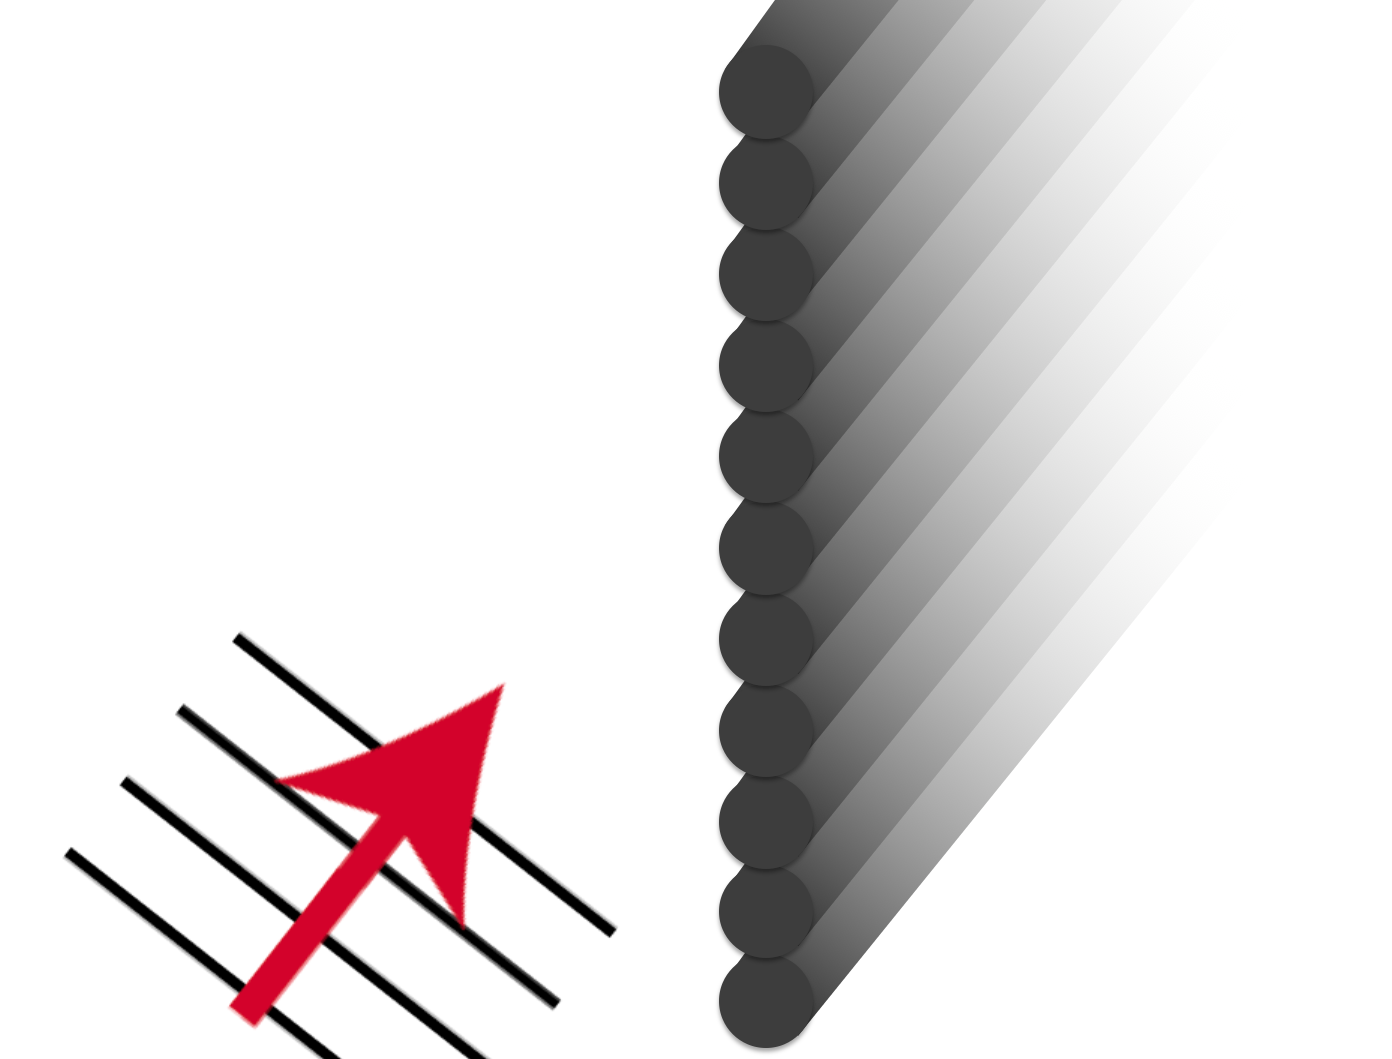
\includegraphics[width=0.3\linewidth]{../diagram/omni-dir03}}
    \caption{A) A ``point absorber'' type omni-directional WEC is denoted as a black circle. B) Though a single ``point absorber'' does not care about wave-direction, an array of such devices does because individual devices shadow one-another depending on wave direction. C) Shadowing is indicated explicitly in this case where the array is a line of ``point absorbers' spaced close enough to capture all incoming energy.\note{These figures are place-holders for now. }}
    \label{fig:omni-dir}
\end{figure}

\subsection{A detailed discussion of the `one-way' approach to estimating the remote resource}

The one-way approach to estimating $R_r$ deserves some explanation because it deviates from the traditional definition of a line-integral. In a traditional line-integral the directionality coefficient is simply:
\begin{align}
    \delta_{*} = \cos(\theta_n - \theta)
    \label{eqn:trad-def}
\end{align}
The primary problem with this definition for the purposes of wave resource assessment is that waves that propagate away from the shoreline of interest ($|\theta_n - \theta|>90$) are subtracted from the resource total. To avoid this we utilize the `one-way' condition for summing wave energy:
\begin{align}
    \delta_1 = 
    \begin{cases}
     \delta_* & \mathrm{for\ }|\theta_n - \theta|<90^\circ \\
    0 & \mathrm{otherwise}.
    \end{cases}
    \label{eqn:1way-def}
\end{align}

The primary draw-back to the one-way condition is that if wave energy criss-crosses back-and-forth across the integration contour, then it is added to the total each time it crosses the contour (rather than being counted, correctly, exactly once). However, since waves do not typically swerve back and forth (i.e., across a straight line), this should only be an issue when the integration contour zig-zags or otherwise has segments that a straight-travelling wave would cross multiple times (e.g., where the contour folds, or when islands are spaced such that there are several independent contours nearby one another).

In order to investigate the extent of double-counting due to the one-way condition, we also keep track of the offshore propagating wave energy using the complimentary definition of the directionality coefficient:
\begin{align}
  \label{eqn:1way-off-def}
    \delta_{off} = 
    \begin{cases}
     -\delta_* & \mathrm{for\ }|\theta_n - \theta|>90^\circ \\
    0 & \mathrm{otherwise}.
    \end{cases}
\end{align}
Where the minus sign makes the value of $\delta_{off}$ positive. We then o

Accounting for both the onshore \eqref{eqn:1way-def} and offshore \eqref{eqn:1way-off-def} wave energy flux independently, gives us the opportunity to assess the relative importance of 

In weighing the pros/cons of these definitions of $\delta$ it is important to understand that wave resource assessments are typically based on models that do not extract wave energy when it encounters the integration contour of interest (e.g., $\leez$). That is, wave energy that propagates across the integration contour at one location might propagate across it again at another location, and there is typically no way to `track' waves (i.e., wave energy) within these models.
This means that both of the definitions of $\delta$ in \eqref{eqn:2way-def} and \eqref{eqn:1way-def} will `double-count' waves that criss-cross back-and-forth across the integration countour ($\delta_2$ to a larger degree). This can occur for waves that travel straight across a zig-zagging integration contour, or for waves that zig-zag along a straight contour. 

\begin{figure}[ht]
    \centering
    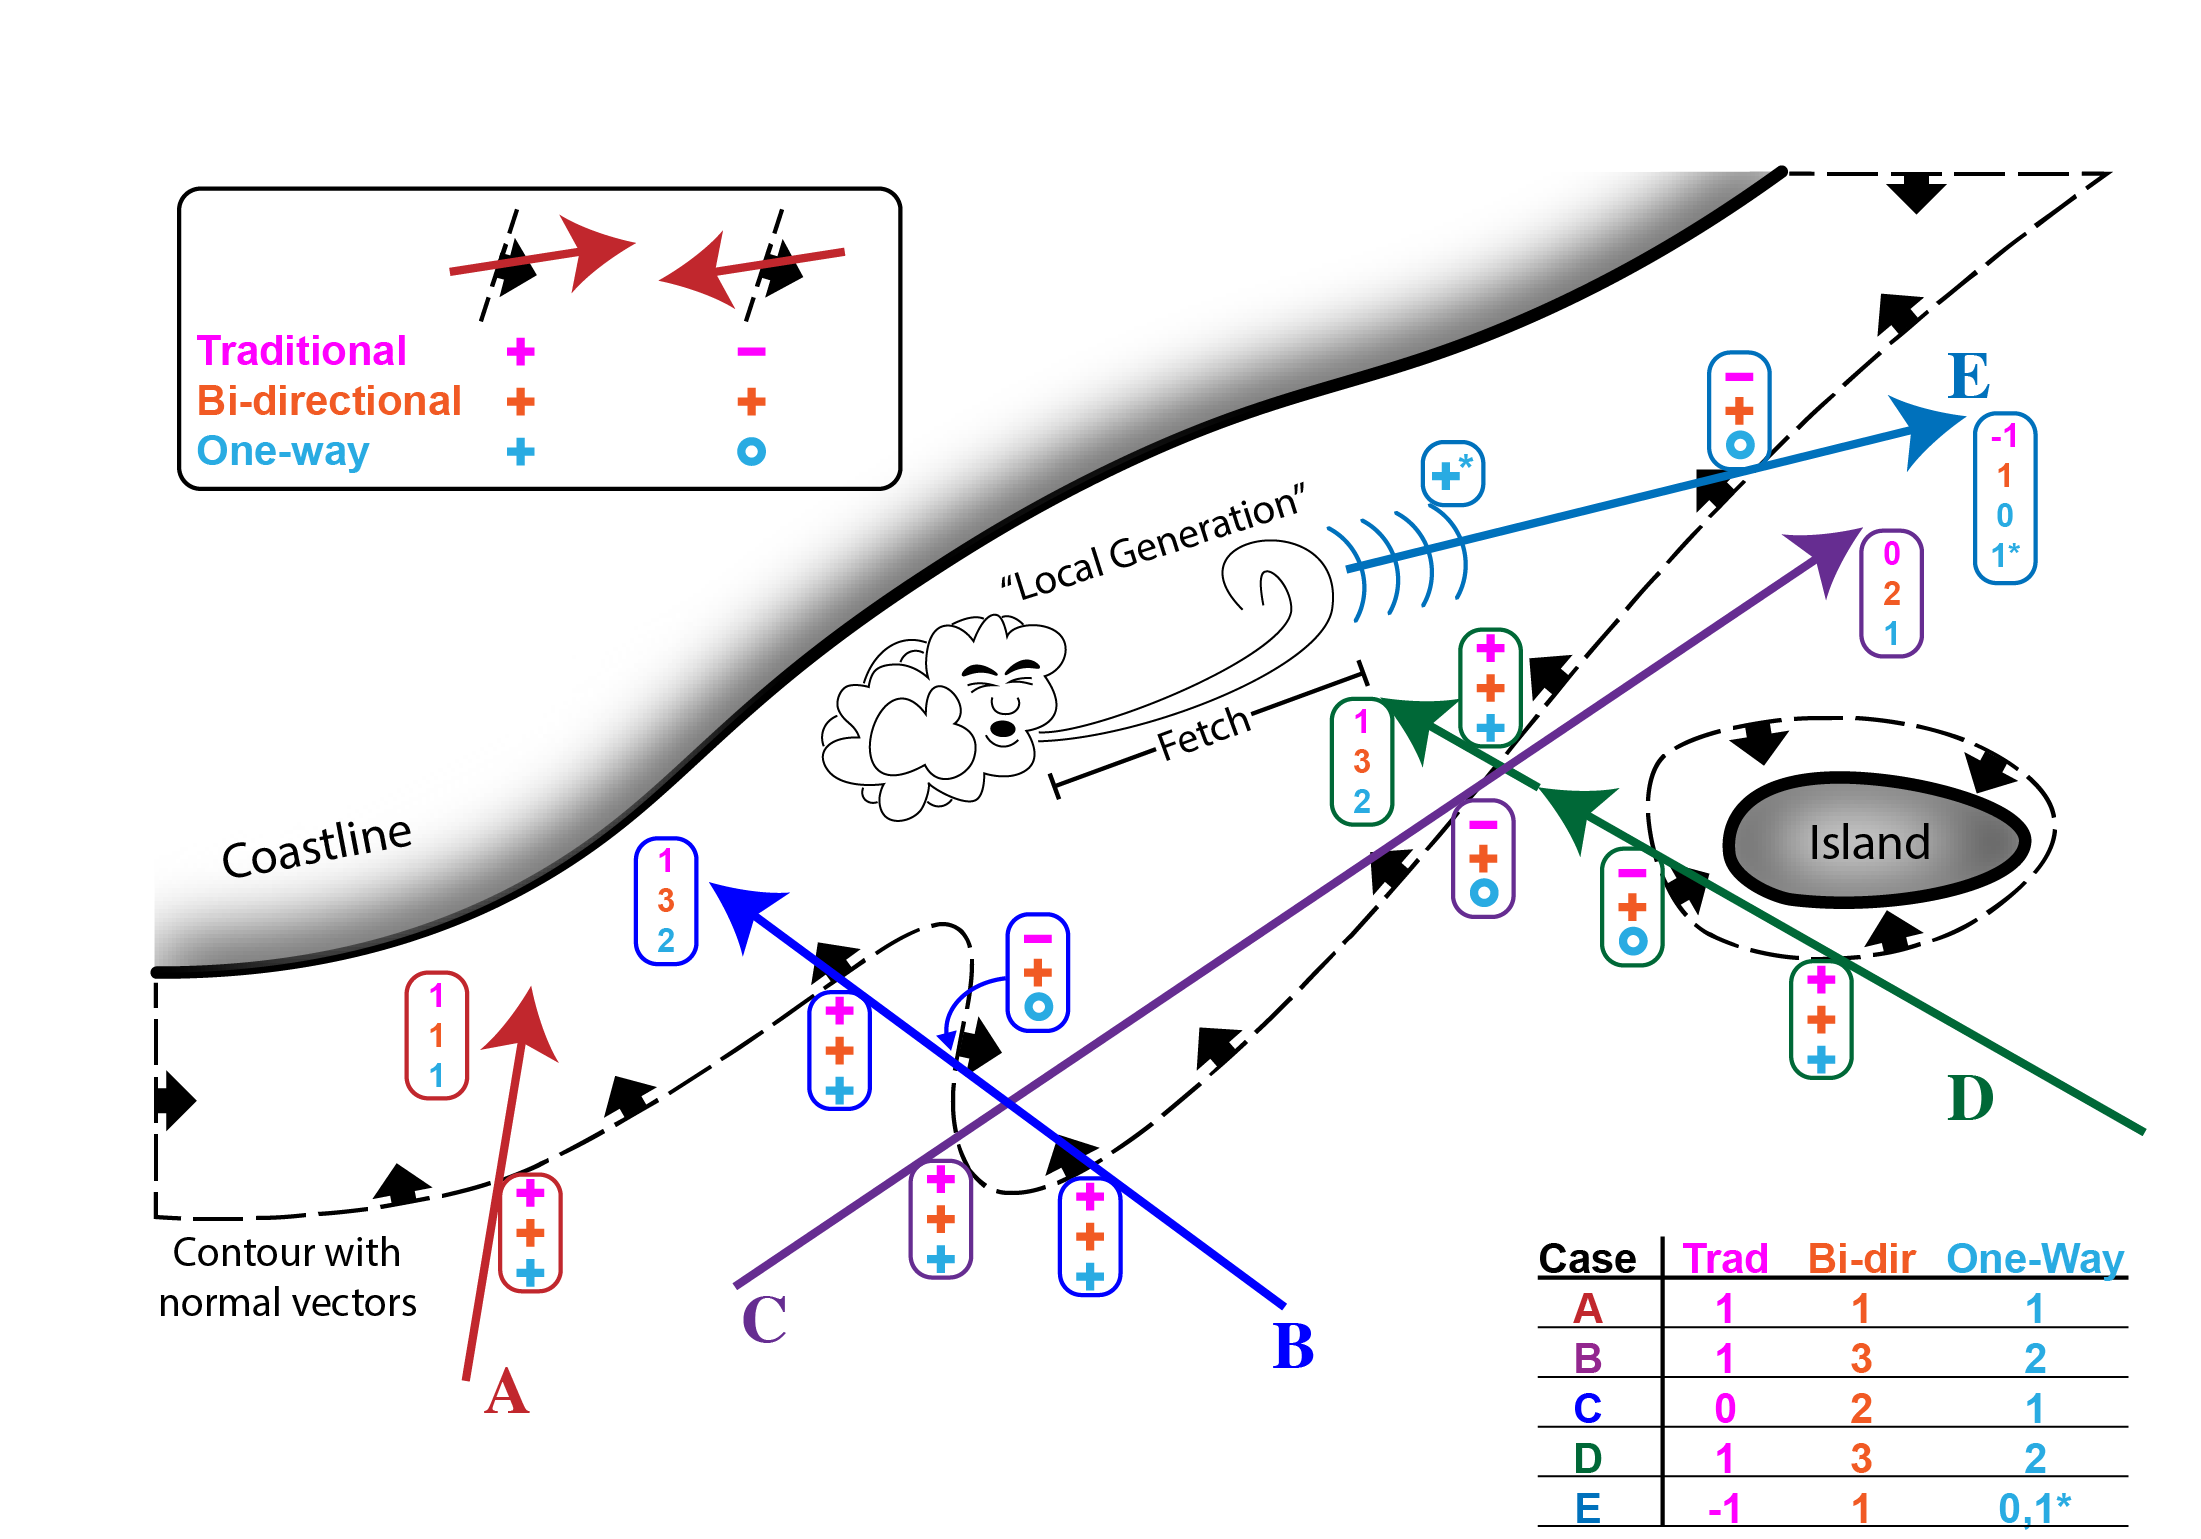
\includegraphics[width=\linewidth]{../diagram/Schematic-Seq01FINAL.png}
    \caption{A diagram depicting different cases of waves (color arrows) crossing an arbitrary integration contour (black dashed line). Black arrows along the contour indicate the contour-normal direction. The upper-left legend — and the boxes along the arrows' lengths — indicate whether energy is added to, subtracted from, or not included in the total depending on the summation method (pink: traditional, orange: bi-directional, cyan: one-way) and direction of wave crossing relative to contour. Boxes at the tip of each arrow indicate the number of times each wave was counted using each method, and the table at lower-right summarizes the totals. A `blowing cloud' image indicates the generation of `local waves' over the region bounded by the integration contour. \note{Need to add a row $E^\dagger$}}
    \label{fig:one-way-diagram}
\end{figure}

Figure \ref{fig:one-way-diagram} provides a schematic of several distinct cases of wave energy (color arrows) propagating across an arbitrary integration contour (black dashed line). Arrow `A' (red) indicates the simplest case of a wave train crossing the contour once before dissipating at the coastline. In this case, all three definitions of $\delta$ give the same correct result of counting this wave exactly once. Arrow `B' (blue) is the case where a wave crosses a zig-zagging countour several times, and shows that $\delta_1$ and $\delta_2$ double-count and triple-count this wave. Arrow `C' (purple) is a case where a wave propagates into and out-of the integration boundary, demonstrating that the $\delta = \delta_*$ does not count this wave, $\delta_1$ counts it once, and $\delta_2$ double-counts it. Arrow `D' (green) is the case of a wave propagating through an island's contour before entering the mainland contour, with essentially the same result as wave `B'. It is also interesting to consider the case where wave `D' does not enter the mainland contour (i.e., if the island is far from shore), in which case the results are the same as wave C.

Finally, this brings us to case `E' where a wave is generated inshore of the boundary and propagates offshore. In this case the wave's energy is subtracted from the total for the traditional case, not counted for the one-way case, and added once (correctly) for the bi-directional method. Note that this is the only case—other than simple case (A)—where the bidirectional method delivers the correct result. When the one-way method is used in conjunction with the local resource method, this waves' energy is included in the total.
When the local resource is added to the numbers in row E, this wave's energy is counted again, which yields row E$^\dagger$.

Importantly, the table in Figure \ref{fig:one-way-diagram} shows that none of the methods defined by the definitions of $\delta$ deliver an accurate estimate of the wave resource for all possible wave paths and integration contours. The only way to avoid double-counting completely is to extract wave energy at the integration contour so that it does not propagate to a different point on the contour where it could be double-counted (or subtracted, depending on the choice of $\delta$). This approach, however, is technically challenging and reduces the flexibility of data analysis (i.e., simulations must be run for each integration contour the user wishes to investigate).

Instead, it is worthwhile to note that $\delta_*$ will provides a lower-bound estimate of $R_r$ (all values are $\le 1$ in the table on Figure \ref{fig:one-way-diagram}), the bidirectional method provides an upper-bound (values $\ge 1$), and the one-way method provides a `best-estimate'. The one-way method is especially accurate when the local waves are accounted for independently (i.e., as $R_l$), as indicated by the `$1^*$' in Figure \ref{fig:one-way-diagram}. Also, the one-way method only over-estimates when waves criss-cross into the boundary multiple times. As long as integration contours are not zig-zagged and assuming waves do not themselves zig-zag across the boundary (i.e., assuming wave turning is not a major issue at the scale and water depth of the integration contour), then the one-way method in conjunction with $R_l$, is a reasonably accurate estimate of the total theoretical resource ($R_t$).

\note{Should we include a table of the different estimates of $R_r$ (e.g., for the west coast) using different definitions of $\delta$?}
\note{What about saying something about the cases where we extracted energy to quantify directional error in remote resource related to one-way method?}

\note{Add a comparison of the one-way method and the unit-circle method, using OUR EEZ boundary (rather than trying to compare with EPRI 2011).}

%%% Local Variables:
%%% TeX-master: "wave_res"
%%% End:
